\documentclass[10pt,twocolumn]{article}

% --- arXiv-compatible typography and layout ---
\usepackage[utf8]{inputenc}
\usepackage[T1]{fontenc}
\IfFileExists{newtxtext.sty}{\usepackage{newtxtext,newtxmath}}{\usepackage{lmodern}}
\usepackage[scaled=0.94]{helvet}
\usepackage[letterpaper,margin=1in]{geometry}
\usepackage{microtype}
\usepackage[table]{xcolor}
\usepackage{graphicx}
\usepackage{booktabs}
\usepackage{array}
\usepackage{tabularx}
\usepackage{enumitem}
\usepackage{amsmath}
\usepackage{hyperref}
\usepackage{xurl}
\usepackage{listings}
\usepackage{caption}
\usepackage[section]{placeins}
\usepackage{balance}
\usepackage{tikz}
\usepackage{pgfplots}
\pgfplotsset{compat=1.18}
\usetikzlibrary{arrows.meta,positioning,fit,calc}

% --- Color system ---
\definecolor{pilotnavy}{HTML}{0B1220}
\definecolor{pilotink}{HTML}{111827}
\definecolor{pilotmuted}{HTML}{526070}
\definecolor{pilotline}{HTML}{D6DEE8}
\definecolor{pilotpaper}{HTML}{F8FAFC}
\definecolor{pilotblue}{HTML}{2563EB}
\definecolor{pilotcyan}{HTML}{0891B2}
\definecolor{pilotgreen}{HTML}{059669}
\definecolor{pilotorange}{HTML}{D97706}
\definecolor{pilotred}{HTML}{DC2626}
\definecolor{pilotviolet}{HTML}{7C3AED}
\definecolor{codebg}{HTML}{F3F6FA}

\pgfplotsset{
    pilot clean axis/.style={
        axis x line*=bottom,
        axis y line*=left,
        axis line style={draw=black!45,line width=0.35pt},
        tick style={draw=black!35,line width=0.35pt},
        tick label style={font=\footnotesize\sffamily,text=pilotmuted},
        label style={font=\footnotesize\sffamily,text=pilotink},
        ymajorgrids=true,
        grid style={draw=pilotline!62,line width=0.3pt},
        scaled ticks=false,
        clip=false,
        every axis plot/.append style={line join=round,line cap=round},
    },
    pilot bar labels/.style={
        nodes near coords,
        every node near coord/.append style={
            font=\scriptsize\sffamily,
            text=pilotink,
            anchor=west,
            xshift=2pt,
        },
    },
}

\hypersetup{
    colorlinks=true,
    linkcolor=pilotblue,
    urlcolor=pilotblue,
    citecolor=pilotblue,
    pdftitle={The Autonomous Agent App Store},
    pdfauthor={Teodor-Ioan Calin},
}

\setlength{\parindent}{15pt}
\setlength{\parskip}{0pt}
\setlength{\emergencystretch}{3em}
\setlength{\columnsep}{0.24in}
\renewcommand{\arraystretch}{1.08}
\setlist[itemize]{leftmargin=1.25em,itemsep=0.25em,topsep=0.25em}
\setlist[enumerate]{leftmargin=1.35em,itemsep=0.25em,topsep=0.25em}
\setlist[description]{leftmargin=1.4em,style=nextline,font=\normalfont\bfseries}

% --- Caption and code style ---
\captionsetup{font=footnotesize,labelfont=bf,textfont=footnotesize,skip=0.3em}
\setlength{\floatsep}{0.7\baselineskip plus 2pt minus 2pt}
\setlength{\textfloatsep}{0.8\baselineskip plus 2pt minus 2pt}
\setlength{\intextsep}{0.8\baselineskip plus 2pt minus 2pt}
\makeatletter
\setlength{\@fptop}{0pt}
\setlength{\@fpsep}{0.9\baselineskip plus 2pt}
\setlength{\@fpbot}{0pt plus 1fil}
\makeatother

\lstdefinestyle{pilot}{
    backgroundcolor=\color{codebg},
    basicstyle=\ttfamily\scriptsize,
    breaklines=true,
    frame=single,
    rulecolor=\color{pilotline},
    framerule=0.4pt,
    xleftmargin=0.2em,
    xrightmargin=0.2em,
    aboveskip=0.45em,
    belowskip=0.35em,
    showstringspaces=false,
    columns=fullflexible,
}
\lstset{style=pilot}

\newcolumntype{Y}{>{\raggedright\arraybackslash}X}
\newcolumntype{R}[1]{>{\raggedleft\arraybackslash}p{#1}}
\newcommand{\pilot}{Pilot Protocol}
\newcommand{\director}{Pilot Director}
\newcommand{\app}[1]{\texttt{#1}}

\title{\textbf{The Autonomous Agent App Store}\\
\large Signed Telemetry, Capability Planning, and Early Adoption in Pilot Protocol}
\author{Teodor-Ioan Calin\\
Pilot Protocol\\
\texttt{teodor@pilotprotocol.network}}
\date{July 2026}

\begin{document}
\maketitle

\begin{abstract}
Autonomous agents increasingly require capabilities that are not built into their base runtime: search, browser automation, secure code execution, data stores, payments, market data, and domain-specific APIs. Human app stores solve a related distribution problem, but an agent app store has a different primary consumer: an agent that discovers and provisions typed capabilities for a task. This paper presents an empirical study of the \pilot{} app store and its planning front end, \director{}, using raw rows from the BigQuery table \texttt{telemetry.events} over a 23-day window from \mbox{2026-06-16} through \mbox{2026-07-08}. The analysis focuses on 268,731 discovery-and-install rows: 150,489 catalogue views, 84,216 app detail views, and 34,026 installs. We describe how Pilot exposes installable capability apps with metadata, manifests, permissions, and typed method schemas; how the protocol supports catalogue discovery, detail inspection, and local provisioning; and how \director{} maps natural-language goals onto validated plans over service agents and app-store methods. The aggregate evidence shows substantial early interest in research, execution, database, market, and security capabilities, with a 55.96\% detail-to-catalogue volume ratio and a 40.40\% install-to-detail volume ratio. We argue that autonomous agent app stores should be evaluated as planner-readable capability markets, not only as human-facing distribution channels.
\end{abstract}

\noindent\textbf{Keywords:} autonomous agents; app stores; capability discovery; telemetry; agent planning; Pilot Protocol.

\section{Introduction}
\label{sec:intro}

Software app stores were designed around human users: a person searches, reads a listing, installs an application, and later launches it through a graphical interface. Autonomous agents invert much of that model. An agent often begins with a task rather than an app name. It needs to know which capability can satisfy the task, whether that capability is already available, how to install it if necessary, which method to call, what arguments to pass, and which parts of the task should remain in the agent's own runtime. This problem sits at the intersection of tool-using language models, planner-controlled API invocation, and software marketplaces \cite{karpas2022mrkl,yao2023react,schick2023toolformer,patil2024gorilla,rochetTirole2003,jansen2013appstores}.

This paper studies that problem through the \pilot{} app store. Pilot provides a network and runtime layer for autonomous agents. Its app store exposes installable local capability apps, each with metadata, a manifest, permissions, and typed IPC methods. Agents can inspect the catalogue, view an app, install it, and invoke methods with structured JSON. In parallel, \director{} serves as a planning front end: a public service agent and HTTP API that maps a natural-language task onto a validated plan over service agents and app-store methods.

The central claim is that an autonomous agent app store should be evaluated by the interaction chain that precedes and enables action: discovery, detail inspection, installation, schema legibility, and planner guidance. Installs alone are not enough. For agents, a store must expose capabilities in a form that a planner can interpret and a runtime can provision.

The empirical questions are:
\begin{description}
    \item[RQ1.] How does an autonomous agent app store work as a protocol and runtime?
    \item[RQ2.] What signed telemetry can measure app-store adoption without observing message contents?
    \item[RQ3.] Which app-store surfaces and capabilities attract early marketplace interest?
    \item[RQ4.] How does a planning layer such as \director{} guide agents from natural language to executable app-store actions?
\end{description}

The paper contributes:
\begin{itemize}
    \item a systems description of the \pilot{} app-store flow: catalogue, detail view, installation, manifest permissions, and supervisor-mediated method access;
    \item a methodology for signed, pseudonymous, event-level telemetry over app-store interactions;
    \item a primary empirical analysis of 268,731 raw discovery-and-install rows from \texttt{telemetry.events};
    \item a description of \director{} as the instruction-generation layer that turns a task into validated calls over both service agents and app-store methods;
    \item limitations and threats to validity covering consent, pseudonymity, payload looseness, and measurement bias.
\end{itemize}

\section{Related Work}
\label{sec:related}

\paragraph{Tool-using language models.}
The literature on tool use has moved from modular architectures that route language-model requests to specialized components \cite{karpas2022mrkl} toward agents that interleave reasoning and actions \cite{yao2023react}, learn when and how to call simple APIs \cite{schick2023toolformer}, and generate API calls over large tool collections \cite{patil2024gorilla}. API-centric benchmarks and training corpora further formalize planning, retrieval, argument construction, execution, and error recovery as separate capabilities \cite{li2023apibank,qin2023toollm,song2023restgpt}. Multi-tool systems such as HuggingGPT show a related pattern in which a language model acts as a controller over a catalogue of specialist models \cite{shen2023hugginggpt}. This paper differs by studying an operational app-store substrate and its observed adoption rather than only model accuracy on benchmark tasks.

\paragraph{Autonomous agent evaluation and orchestration.}
Agent benchmarks increasingly emphasize long-horizon tasks, interactive environments, and functional success rather than static text generation. WebArena constructs realistic web environments with task-level success criteria \cite{zhou2023webarena}, while AgentBench evaluates LLM agents across multiple interactive environments \cite{liu2023agentbench}. Planner and orchestration systems provide a complementary line of evidence: SayCan grounds language-model planning in feasible skills \cite{ahn2022saycan}, Voyager accumulates an executable skill library through exploration \cite{wang2023voyager}, AutoGen composes multiple conversable agents with tools and code execution \cite{wu2023autogen}, and generative agents show how memory and planning can produce autonomous behavior over time \cite{park2023generativeagents}. These systems motivate a capability-market perspective: for agents, a store must make tools discoverable, installable, permissioned, and legible to planners.

\paragraph{App stores and platform economics.}
Human app stores are commonly understood as curated marketplaces and two-sided platforms connecting developers and users \cite{rochetTirole2003,jansen2013appstores}. Software-engineering work has mined app stores for ratings, reviews, releases, metadata, and ecosystem structure \cite{harman2012appstoremining,martin2017appstoreanalysis,zhu2024appstore}. The autonomous-agent app store differs in the identity of the consumer and in the presentation of demand: the store must be readable both to humans and to planners that select capabilities on behalf of agents.

\paragraph{Telemetry, signatures, and privacy boundaries.}
Signed telemetry uses cryptographic authenticity, here Ed25519 as standardized in RFC 8032 \cite{rfc8032}, but authenticity is not the same as identity, consent, or anonymity. NIST guidance on personally identifiable information and de-identification frames why pseudonymous operational identifiers still require careful interpretation \cite{nist800122,nistir8053}. Classical privacy work on $k$-anonymity and de-anonymization further cautions that pseudonymous records can remain linkable when auxiliary information is available \cite{sweeney2002kanonymity,narayanan2008deanonymization}. This study presents aggregate adoption measures and does not claim formal differential privacy in the sense of Dwork et al. \cite{dwork2006}.

\section{System Overview}
\label{sec:system}

\subsection{The App Store as an Agent Capability Substrate}

The \pilot{} app store exposes capabilities as installable local apps. An app is not primarily a visual interface; it is a capability provider. Once installed, it can be supervised by the daemon and invoked over local IPC through named methods. This makes it suitable for autonomous agents, which can treat each app as a typed service \cite{pilotProtocolSource}.

This design follows the broader shift from monolithic model inference toward systems that bind language models to external modules, tools, and APIs \cite{karpas2022mrkl,schick2023toolformer,patil2024gorilla}. Recent protocol work such as the Model Context Protocol similarly emphasizes standardized connections between LLM applications, tools, and external data sources \cite{mcp2025spec}. The app-store distinction is that tools are not only prompt-time affordances; they are installable, permissioned, versioned local capabilities.

At the command surface, the core workflow is compact:

\begin{lstlisting}[language=bash]
pilotctl appstore catalogue
pilotctl appstore view io.pilot.cosift
pilotctl appstore install io.pilot.cosift
pilotctl appstore call io.pilot.cosift cosift.search '{"q":"..."}'
\end{lstlisting}

The catalogue and view flows expose metadata. The install flow writes the app bundle to the local app root and records an install. The call flow connects to the app's Unix socket and invokes a named method with JSON arguments. The daemon-side supervisor enforces that a method is exposed by the target manifest, and for cross-app calls it checks that the caller holds an \texttt{ipc.call} grant for the target method. This creates an app-store model built for agents: discovery and installation are explicit, while execution is typed, permissioned, and callable from automation.

\subsection{Service Agents and App-Store Apps}

\pilot{} exposes two capability surfaces. The first is a network of service agents, invoked over the overlay with \texttt{pilotctl send-message}. The second is the local app-store method surface, invoked with \texttt{pilotctl appstore call}. \director{} normalizes both into a single capability catalogue. This resembles API-selection and tool-retrieval settings studied in API-Bank, ToolLLM, RestGPT, and Gorilla, but here the planner targets a live runtime surface rather than a benchmark-only tool list \cite{li2023apibank,qin2023toollm,song2023restgpt,patil2024gorilla}. A capability record is either an agent or an app method:

\begin{lstlisting}
agent:
  pilotctl send-message <id> --data '/data {...}' --wait

app-method:
  pilotctl appstore call <app> <method> '{...}'
\end{lstlisting}

This distinction matters because service agents and local apps occupy different trust and execution positions. Service agents are remote actors reachable through the Pilot overlay. App-store apps are local capabilities installed on the user's machine and mediated by local runtime policy. The planner can select either, depending on the task, availability, and required capability.

\begin{figure*}[!t]
\centering
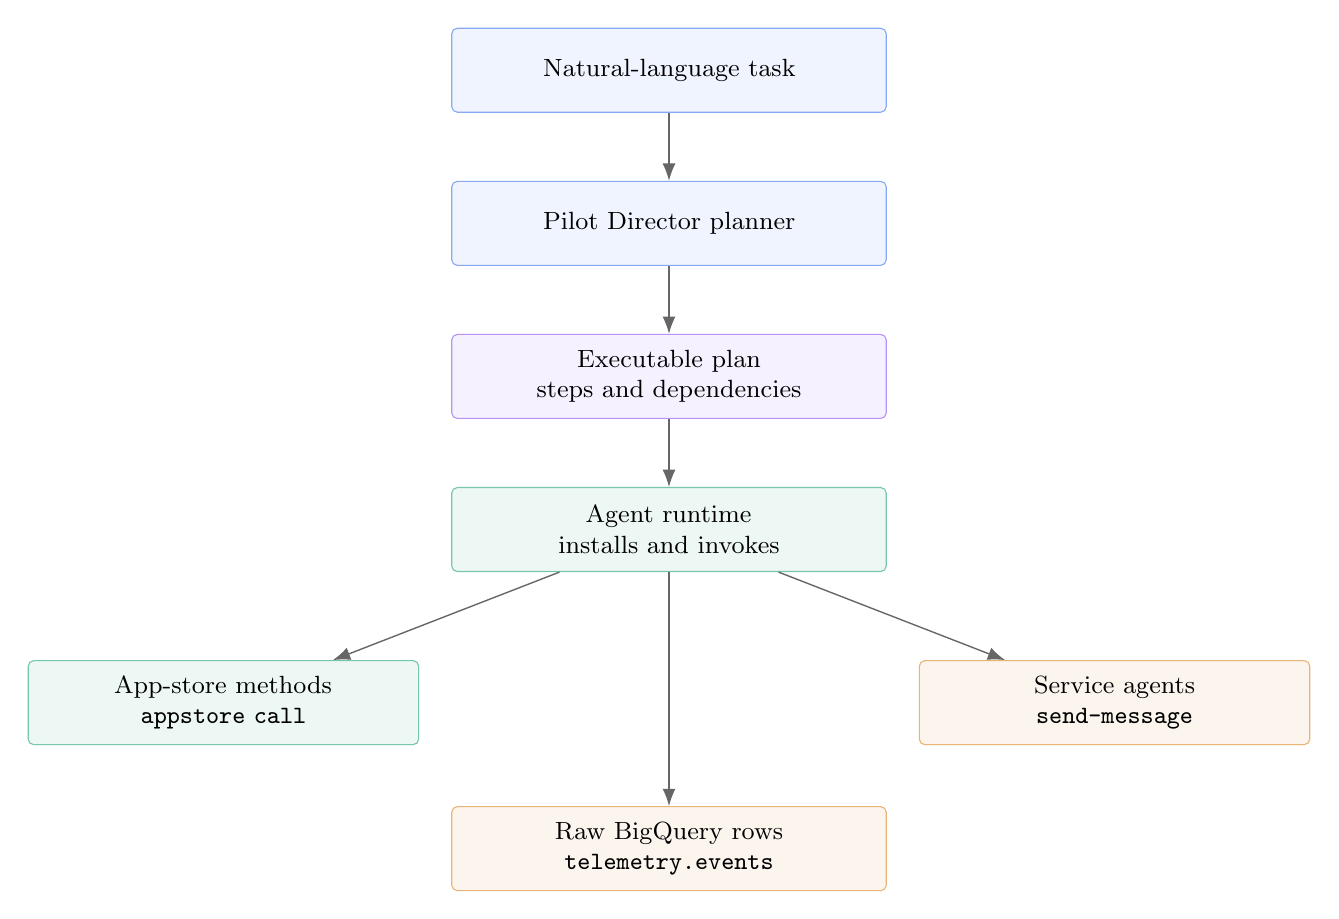
\begin{tikzpicture}[
  node distance=0.34in,
  box/.style={draw=pilotline,rounded corners=2pt,fill=white,minimum height=0.42in,align=center,text width=2.08in,font=\small},
  branch/.style={box,text width=1.86in},
  blue/.style={draw=pilotblue!55,fill=pilotblue!7},
  green/.style={draw=pilotgreen!55,fill=pilotgreen!7},
  orange/.style={draw=pilotorange!55,fill=pilotorange!7},
  violet/.style={draw=pilotviolet!55,fill=pilotviolet!7},
  arrow/.style={-{Latex[length=2.2mm]},draw=black!60,line width=0.5pt}
]
\node[box,blue] (task) {Natural-language task};
\node[box,blue,below=of task] (director) {\director{} planner};
\node[box,violet,below=of director] (plan) {Executable plan\\steps and dependencies};
\node[box,green,below=of plan] (runtime) {Agent runtime\\installs and invokes};
\node[branch,green,below left=0.44in and 0.16in of runtime] (apps) {App-store methods\\\texttt{appstore call}};
\node[branch,orange,below right=0.44in and 0.16in of runtime] (agents) {Service agents\\\texttt{send-message}};
\node[box,orange,below=1.17in of runtime] (bq) {Raw BigQuery rows\\\texttt{telemetry.events}};

\draw[arrow] (task) -- (director);
\draw[arrow] (director) -- (plan);
\draw[arrow] (plan) -- (runtime);
\draw[arrow] (runtime) -- (apps);
\draw[arrow] (runtime) -- (agents);
\draw[arrow] (runtime) -- (bq);
\end{tikzpicture}
\caption{A natural-language request becomes a typed execution plan. \director{} bridges human intent, agent reasoning, local app-store methods, remote service agents, and signed telemetry.}
\label{fig:director-flow}
\end{figure*}

\subsection{\director{} as the Guidance Layer}

\director{} exposes the \href{https://director.pilotprotocol.network/}{director.pilotprotocol.network} endpoint, HTTP \texttt{/api/plan}, and Pilot-overlay entry points \cite{pilotDirector}. A user or agent can request a plan as follows:

\begin{lstlisting}[language=bash]
pilotctl send-message pilot-director \
  --data '/data {"task":"Research a company and summarize risks"}' \
  --wait
\end{lstlisting}

The service parses the task, searches its known capabilities, and emits a plan. Each plan step contains a resource, parameters, dependency references, and an output name. The planner also supports \texttt{handoff} steps for local runtime actions such as notification, scheduling, email, approval, or file generation. A separate \texttt{/api/skill} endpoint can turn a task and successful execution trace into a reusable \texttt{SKILL.md}. In this sense, \director{} is not a marketplace listing page. It is an operational interface that instructs agents how to use the marketplace, echoing prior work on reasoning-and-acting loops and model-controlled tool orchestration \cite{yao2023react,shen2023hugginggpt,zhou2023webarena}.

\section{Telemetry Methodology}
\label{sec:methodology}

\subsection{Event Grammar}

The analysis is based on raw BigQuery rows from \texttt{telemetry.events} \cite{pilotTelemetryBQ}. Each row contains an \texttt{event\_id}, a \texttt{kind}, a timestamp \texttt{ts}, a client-claimed \texttt{node\_id}, a verified public-key \texttt{fingerprint}, a JSON \texttt{payload}, and \texttt{received\_at}. Clients may supply the event identifier; otherwise, the ingestion service generates one. The identifier is also used as the BigQuery streaming insert ID for best-effort retry deduplication. The reported measures count stored rows and therefore do not assume exactly-once delivery. We analyze three discovery-and-install event kinds:

\begin{table*}[!t]
\centering
\caption{Event kinds used in the adoption analysis.}
\label{tab:event-kinds}
\begin{tabularx}{\textwidth}{@{}p{0.2\textwidth}Y Y@{}}
\toprule
\textbf{Kind} & \textbf{Meaning} & \textbf{Primary fields used} \\
\midrule
\texttt{catalogue\_viewed} & Catalogue surface was requested. & timestamp, identity, optional payload app context. \\
\texttt{appstore\_view} & App-store detail or listing view. & app identifier where present, timestamp, identity. \\
\texttt{app\_installed} & App install action was emitted. & \texttt{payload.app\_id}, installer identity. \\
\bottomrule
\end{tabularx}
\end{table*}

The warehouse covers a 23-day observation window from 2026-06-16 through 2026-07-08. Dates are filtered by \texttt{DATE(received\_at)}. Review rows and other event kinds are outside this measurement scope. We exclude \app{io.test.*} app identifiers from per-app install analysis because they are ingestion-test artifacts rather than marketplace demand.

\subsection{Authenticity and Pseudonymity}

Client telemetry is signed with Ed25519, an EdDSA instance standardized by RFC 8032 \cite{rfc8032}. The client sends \texttt{X-Pilot-Timestamp}, \texttt{X-Pilot-Public-Key}, and \texttt{X-Pilot-Signature}. The signed message is:

\begin{lstlisting}
timestamp + "\n" + raw_request_body
\end{lstlisting}

The ingestion service verifies the signature and stores the SHA-256 fingerprint of the public key. The \texttt{fingerprint} is therefore stronger than a raw client string. The \texttt{node\_id}, however, is client-claimed and should be treated as a behavioral identifier rather than a cryptographic identity.

\subsection{Consent and Measurement Boundary}

The CLI telemetry path is controlled by \texttt{\textasciitilde/.pilot/config.json}; telemetry defaults to enabled and can be disabled. Review events use a separate consent path and are not included in the adoption ratios. The analyzed schema stores event metadata and app identifiers, not network addresses or agent message contents. The analysis therefore treats discovery and install telemetry as signed operational records with a specific measurement boundary, not as a complete census of all agent behavior.

The payload schema is intentionally loose. Catalogue events can be broad and may not carry an app identifier, while detail and install events are more often app-specific. We therefore compute robust measures from fields that are consistently useful: event kind, timestamp, identity fingerprints, and app identifier where present.

\section{Adoption Results}
\label{sec:results}

\subsection{Discovery and Provisioning}

The scoped event volume shows an aggregate marketplace progression adapted to agents. Catalogue requests are the broad discovery surface, detail views indicate app-level inspection, and installs indicate local provisioning of a capability. Across 268,731 discovery-and-install rows, detail-view volume equals 55.96\% of catalogue-view volume, and install volume equals 40.40\% of detail-view volume. These are aggregate volume ratios rather than session-linked conversion rates.

\begin{figure}[!htbp]
\centering
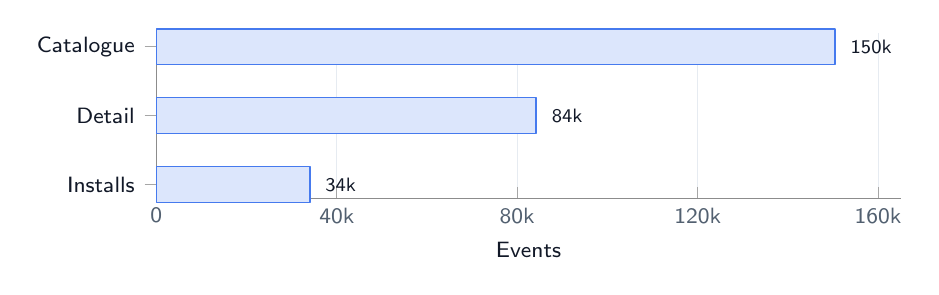
\begin{tikzpicture}
\begin{axis}[
    pilot clean axis,
    pilot bar labels,
    xbar,
    width=0.91\linewidth,
    height=1.45in,
    xmin=0,
    xmax=165000,
    xlabel={Events},
    symbolic y coords={Installs,Detail,Catalogue},
    ytick=data,
    yticklabel style={font=\footnotesize\sffamily,text=pilotink},
    xmajorgrids=true,
    ymajorgrids=false,
    xtick={0,40000,80000,120000,160000},
    xticklabels={0,40k,80k,120k,160k},
    bar width=13pt,
    point meta=explicit symbolic,
    nodes near coords={\pgfplotspointmeta},
]
\addplot+[draw=pilotblue!85,fill=pilotblue!16,line width=0.55pt] coordinates {
    (150489,Catalogue) [150k]
    (84216,Detail) [84k]
    (34026,Installs) [34k]
};
\end{axis}
\end{tikzpicture}
\caption{Aggregate discovery-to-install volume over the 23-day BigQuery window.}
\label{fig:progression}
\end{figure}

\begin{table*}[!t]
\centering
\caption{Headline adoption metrics.}
\label{tab:headline}
\begin{tabularx}{\textwidth}{@{}Y R{1.35in} Y@{}}
\toprule
\textbf{Metric} & \textbf{Value} & \textbf{Interpretation} \\
\midrule
Discovery-and-install rows & 268,731 & Catalogue, detail, and install rows in scope. \\
Catalogue views & 150,489 & Broad app-store discovery surface. \\
Detail views & 84,216 & App-level inspection before install. \\
Installs & 34,026 & Local provisioning events. \\
Detail-to-catalogue ratio & 55.96\% & Detail-view volume divided by catalogue-view volume. \\
Install-to-detail ratio & 40.40\% & Install volume divided by detail-view volume. \\
Install-to-catalogue ratio & 22.61\% & Install volume divided by catalogue-view volume. \\
Top-eight install share & 76.00\% & Share of installs represented by Table~\ref{tab:top-installs}. \\
\bottomrule
\end{tabularx}
\end{table*}

\subsection{Temporal Growth}

Observed volume intensified after the first week. Catalogue and detail activity both rose into Week 27, while installs peaked in Week 26 and remained high in Week 27. Week 28 is a partial week ending on 2026-07-08. Because the warehouse remained live during extraction, its final partial-week values are reconciled to the fixed headline snapshot by subtracting Weeks 25--27 from the window totals. The pattern is consistent with a young marketplace receiving substantial discovery traffic while agents and users continue to evaluate which capabilities merit local provisioning.

\begin{figure}[!htbp]
\centering
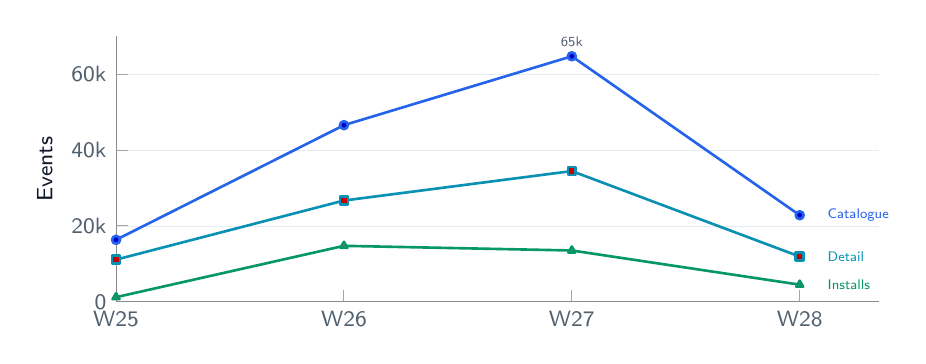
\begin{tikzpicture}
\begin{axis}[
    pilot clean axis,
    width=0.93\linewidth,
    height=1.95in,
    xmin=25,
    xmax=28.35,
    ymin=0,
    ymax=70000,
    ylabel={Events},
    xtick={25,26,27,28},
    xticklabels={W25,W26,W27,W28},
    ymajorgrids=true,
    ytick={0,20000,40000,60000},
    yticklabels={0,20k,40k,60k},
    mark options={scale=0.72},
]
\addplot+[line width=0.95pt,mark=*,color=pilotblue] coordinates {(25,16344) (26,46575) (27,64738) (28,22832)};
\addplot+[line width=0.95pt,mark=square*,color=pilotcyan] coordinates {(25,11121) (26,26701) (27,34469) (28,11925)};
\addplot+[line width=0.95pt,mark=triangle*,color=pilotgreen] coordinates {(25,1221) (26,14757) (27,13531) (28,4517)};
\node[anchor=west,font=\tiny\sffamily,text=pilotblue] at (axis cs:28.08,22832) {Catalogue};
\node[anchor=west,font=\tiny\sffamily,text=pilotcyan] at (axis cs:28.08,11925) {Detail};
\node[anchor=west,font=\tiny\sffamily,text=pilotgreen] at (axis cs:28.08,4517) {Installs};
\node[anchor=south,font=\tiny\sffamily,text=pilotmuted] at (axis cs:27,64738) {65k};
\end{axis}
\end{tikzpicture}
\caption{Weekly discovery and install volume. Week 28 is partial and ends on 2026-07-08.}
\label{fig:weekly}
\end{figure}

\begin{table}[!htbp]
\centering
\caption{Weekly discovery and install totals.}
\label{tab:weekly}
\begin{tabular}{@{}l r r r@{}}
\toprule
\textbf{Week} & \textbf{Catalogue} & \textbf{Detail} & \textbf{Installs} \\
\midrule
W25 & 16,344 & 11,121 & 1,221 \\
W26 & 46,575 & 26,701 & 14,757 \\
W27 & 64,738 & 34,469 & 13,531 \\
W28 & 22,832 & 11,925 & 4,517 \\
\bottomrule
\end{tabular}
\end{table}

\subsection{Installed Capability Mix}

Install volume suggests broad interest in research, coding, database, market, and security-oriented capabilities. The leading install set, shown in Table~\ref{tab:top-installs}, spans retrieval, execution, security, relational storage, market intelligence, analytics, and container workflows. The top entry, \app{io.pilot.cosift}, recorded 5,162 installs and 5,037 unique installer fingerprints. The top eight apps account for 25,860 installs, or 76.00\% of all observed installs.

\begin{table}[!htbp]
\centering
\caption{Top apps by install volume.}
\label{tab:top-installs}
\begin{tabular}{@{}l r r@{}}
\toprule
\textbf{App} & \textbf{Installs} & \textbf{Fingerprints} \\
\midrule
\app{io.pilot.cosift} & 5,162 & 5,037 \\
\app{io.pilot.smolmachines} & 3,986 & 3,966 \\
\app{io.pilot.miren} & 3,496 & 3,458 \\
\app{io.pilot.aegis} & 3,116 & 3,064 \\
\app{io.pilot.postgres} & 3,008 & 2,984 \\
\app{io.pilot.slipstream} & 2,853 & 2,801 \\
\app{io.pilot.duckdb} & 2,723 & 2,687 \\
\app{io.pilot.docker} & 1,516 & 1,509 \\
\bottomrule
\end{tabular}
\end{table}

\begin{figure}[!htbp]
\centering
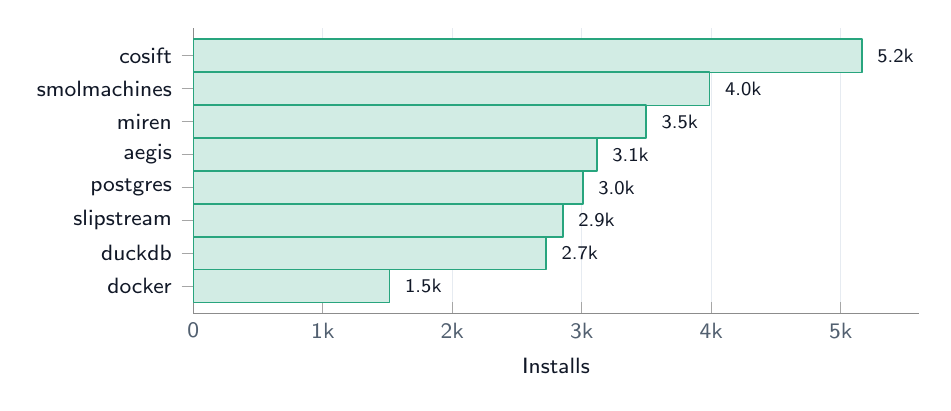
\begin{tikzpicture}
\begin{axis}[
    pilot clean axis,
    pilot bar labels,
    xbar,
    width=0.89\linewidth,
    height=2.05in,
    xmin=0,
    xmax=5600,
    xlabel={Installs},
    symbolic y coords={docker,duckdb,slipstream,postgres,aegis,miren,smolmachines,cosift},
    ytick=data,
    yticklabel style={font=\footnotesize\sffamily,text=pilotink},
    xmajorgrids=true,
    xtick={0,1000,2000,3000,4000,5000},
    xticklabels={0,1k,2k,3k,4k,5k},
    enlarge y limits=0.12,
    ymajorgrids=false,
    bar width=12pt,
    point meta=explicit symbolic,
    nodes near coords={\pgfplotspointmeta},
]
\addplot+[fill=pilotgreen!18,draw=pilotgreen!86,line width=0.55pt] coordinates {
    (5162,cosift) [5.2k]
    (3986,smolmachines) [4.0k]
    (3496,miren) [3.5k]
    (3116,aegis) [3.1k]
    (3008,postgres) [3.0k]
    (2853,slipstream) [2.9k]
    (2723,duckdb) [2.7k]
    (1516,docker) [1.5k]
};
\end{axis}
\end{tikzpicture}
\caption{Top apps by install volume. The leading apps span research, execution, security, storage, market, analytics, and infrastructure categories.}
\label{fig:top-installs}
\end{figure}

\section{The Role of \director{}}
\label{sec:director}

\subsection{From Intent to Calls}

\director{} ties into the app store by translating a task into a plan that an agent can execute. Its output is a typed object with \texttt{steps}, each step containing a \texttt{resource}, \texttt{params}, \texttt{depends\_on}, optional \texttt{uses}, optional \texttt{handoff}, and an \texttt{output} name. The resource can be a network service agent or an app-store method. App-store method calls are rendered as:

\begin{lstlisting}[language=bash]
pilotctl appstore call <app> <method> '{...}'
\end{lstlisting}

Service-agent calls are rendered as:

\begin{lstlisting}[language=bash]
pilotctl send-message <agent-id> --data '/data {...}' --wait
\end{lstlisting}

This matters for adoption because it reduces the cost of capability discovery. An agent need not know every app identifier in advance. It can ask \director{} how to decompose a task, then receive a validated recipe using installed apps, installable apps, remote service agents, and local handoffs.

\subsection{A Planner-Native Marketplace}

Traditional marketplaces optimize for search, rankings, categories, reviews, and install buttons. A marketplace for autonomous agents must expose a second interface: planner-readable affordances. The app's name and description remain useful, but the planner needs method names, parameter schemas, permissions, examples, and invocation syntax. This recasts the app store from a two-sided human marketplace into a tool-selection substrate for agents \cite{rochetTirole2003,jansen2013appstores,qin2023toollm,mcp2025spec}.

\director{} therefore acts as a bridge between discovery and execution:
\begin{enumerate}
    \item The user or agent gives a natural-language goal.
    \item The planner maps the goal onto known capabilities.
    \item The plan emits concrete calls over \texttt{pilotctl appstore call} or \texttt{pilotctl send-message}.
    \item The runtime executes the plan, installs missing local apps where appropriate, and emits signed events.
    \item Successful traces can be promoted into reusable skills through \texttt{/api/skill}.
\end{enumerate}

This loop explains why the app store and \director{} should be studied together. The store supplies the capabilities; \director{} supplies the operational grammar that helps agents choose and use them.

\section{Discussion}
\label{sec:discussion}

\subsection{Observed Capability Demand}

The install pattern points to several agent-native demand categories.

\begin{description}
    \item[Research and retrieval.] The leading install table starts with a research and retrieval capability, suggesting early demand for information gathering, search, and synthesis.
    \item[Execution.] The second-ranked app is an execution-oriented capability, indicating interest in controlled computation or code execution as an agent primitive.
    \item[Data and infrastructure.] Database, analytics, and container apps appear in the top install set, consistent with agents assembling local data and runtime toolchains.
    \item[Market and security capabilities.] Market-intelligence and security-oriented tools are also salient in early provisioning.
\end{description}

The install mix is broad rather than single-purpose. The leading eight apps include research, execution, database, market, analytics, security, and container capabilities. This is consistent with an agent marketplace in which the app store is less a catalogue of end-user applications than a provisioning surface for composable capabilities.

\subsection{Task-Conditioned Adoption}

Agent app-store adoption is task-conditioned rather than preference-driven. An agent does not install a capability because it wants an app in the consumer sense; it installs because a current or anticipated task exposes a missing typed affordance. The present event grammar does not label task intent, but the installed capability mix motivates three analytical demand regimes.

\begin{description}
    \item[Operator-directed one-off tasks.] These begin with a concrete user request: research this entity, inspect this code path, run this computation, query this dataset, or assess this risk. They often have high immediate marginal value because intent is already supplied, success can be judged locally, and the cost of provisioning a capability is tied to a specific outcome.
    \item[Recurring workflows.] These include scheduled monitoring, periodic refresh, repeated retrieval, or background checks. They can be valuable, but their value is delayed and depends on reliability, state, idempotence, notifications, approvals, and failure recovery. A recurring workflow is therefore a weaker early install signal unless the store and planner can make recurrence trustworthy.
    \item[Infrastructure provisioning.] Database, analytics, and container capabilities behave like option value. They may not satisfy a user request by themselves, but they expand the set of future tasks an agent can perform.
\end{description}

Task horizon therefore changes how adoption should be read. Operator-directed one-offs have immediate, attributable value because demand and a success criterion already exist. Recurring workflows have contingent value, discounted by schedule state, permission persistence, drift, cost, and interruption handling. Infrastructure provisioning has option value because it enlarges the future task frontier. For autonomous agent stores, the highest-value early demand may therefore come from capabilities that complete concrete user-directed tasks, while recurring workflows require stronger product primitives before their value is fully visible.

\subsection{Planner-Readable Demand as Market Signal}

Human app stores often rely on downloads, ratings, revenue, and active-device metrics \cite{harman2012appstoremining,martin2017appstoreanalysis}. Autonomous agent app stores add a different market signal: whether a capability is represented in a form that an agent or planner can discover, inspect, provision, and reason about. That view can support:

\begin{itemize}
    \item capability ranking based on discovery-to-install volume ratios;
    \item planner optimization, where \director{} can prefer apps with clear schemas and demonstrated install interest;
    \item developer feedback about which listings, permissions, examples, and schemas agents actually understand;
    \item security and permission review for sensitive capability surfaces;
    \item marketplace economics based on provisioning, trust, and planner compatibility.
\end{itemize}

This paper does not claim that install volume alone is quality. Install volume can reflect curiosity, default placement, documentation, planner recommendations, or genuine capability demand. The key point is that app-store telemetry makes early marketplace movement observable without inspecting message contents, while remaining explicit about the difference between aggregate volume ratios and user-level conversion.

\subsection{Data Quality Observations}

Two attribution gaps are visible. First, 94,473 catalogue-view events and 6,558 store-view events have no app attribution. This is expected for broad catalogue views but less useful for listing-level analysis. Second, 58 install events lack \texttt{app\_id}. These missing fields are small relative to total installs but should be addressed for stricter future progression analysis.

The dataset also contains \app{io.test.*} app identifiers. These were excluded from per-app analysis as ingestion-test artifacts. The exclusion does not affect headline event-kind totals, but it matters for ranking real app demand.

\section{Threats to Validity}
\label{sec:validity}

\textbf{Identity is pseudonymous.} A fingerprint identifies a public key seen by telemetry, not a person. A node ID is client-claimed. Distinct fingerprints and node IDs can overcount or undercount real agents depending on key rotation, reinstallation, local configuration, and multi-agent setups. This is why the paper treats fingerprints as operational identifiers rather than as natural persons or organizations, following privacy guidance that distinguishes pseudonymous and linkable data from anonymous data \cite{nist800122,nistir8053}.

\textbf{Consent paths are not perfectly uniform.} The CLI has an opt-out configuration. Review events use separate consent and are outside the volume ratios. This paper therefore treats the data as signed operational telemetry with known boundaries, not as a complete census of all agent behavior.

\textbf{Payload schema is loose.} App IDs are extracted from JSON payload fields. Missing or inconsistent payload fields can affect app-level aggregates.

\textbf{The window is early and short.} The 23-day window captures early adoption dynamics. It is enough to observe strong signals, but not enough to claim long-term retention, seasonality, or equilibrium marketplace behavior.

\textbf{Guidance can shape demand.} If \director{} or other examples recommend certain apps, observed installs may reflect planner guidance as well as independent agent preference. For autonomous systems, this is not a defect; it is part of the phenomenon being measured.

\section{Implications for Agent App Stores}
\label{sec:implications}

The results suggest six design principles.

\begin{enumerate}
    \item \textbf{Instrument discovery and provisioning.} Catalogue, detail, and install events measure aggregate movement from awareness to local capability setup.
    \item \textbf{Model task shape as demand.} Operator-directed one-offs, recurring workflows, and infrastructure provisioning have different value curves and should not be collapsed into a single adoption score.
    \item \textbf{Expose planner-readable schemas.} App-store metadata should be legible to agents and planners, not only humans.
    \item \textbf{Separate identity claims from verified keys.} Cryptographic fingerprints are more reliable than client-claimed node IDs, but both have analytical value when interpreted carefully.
    \item \textbf{Treat missing attribution as a product issue.} Catalogue-level browsing can be anonymous to an app, but detail and install events should preserve app identifiers consistently.
    \item \textbf{Study planners and stores together.} A planner such as \director{} changes how agents discover and use capabilities; adoption is partly a function of guidance quality.
\end{enumerate}

\section{Conclusion}
\label{sec:conclusion}

The \pilot{} app store shows how an autonomous agent marketplace can function as more than a distribution channel. It is a capability substrate: agents discover apps, inspect their affordances, and provision typed tools for future work. Across 268,731 raw BigQuery rows from 2026-06-16 through 2026-07-08, we observe a clear progression from catalogue browsing to detail views and installs. The strongest install signals concentrate in apps that expose research, execution, database, market, security, and infrastructure capabilities.

\director{} completes the picture. It maps natural-language tasks onto validated plans over service agents and app-store methods, giving agents the procedural instructions needed to navigate the marketplace. This turns the app store from a passive catalogue into an active coordination layer. For autonomous agents, adoption is not simply what gets downloaded; it is what becomes legible, trusted, and provisioned for a task. This is task-conditioned adoption. The most valuable early tasks may be concrete, operator-directed one-offs; recurring workflows become valuable when the store and planner can also carry state, schedules, approvals, and recovery.

\FloatBarrier
\balance
\appendix

\section{Representative BigQuery Queries}
\label{app:sql}

The following queries illustrate the measurement procedures used for the aggregates in this paper. They are included for methodological transparency and are intentionally written against the raw \texttt{telemetry.events} table.

\subsection{Event-Kind Totals}

\begin{lstlisting}[language=SQL]
SELECT
  kind,
  COUNT(*) AS events
FROM `telemetry.events`
WHERE DATE(received_at) BETWEEN '2026-06-16' AND '2026-07-08'
  AND kind IN (
    'catalogue_viewed',
    'appstore_view',
    'app_installed'
  )
GROUP BY kind
ORDER BY events DESC;
\end{lstlisting}

\subsection{Installs by App}

\begin{lstlisting}[language=SQL]
SELECT
  JSON_VALUE(payload, '$.app_id') AS app_id,
  COUNT(*) AS installs,
  COUNT(DISTINCT fingerprint) AS unique_fingerprints
FROM `telemetry.events`
WHERE DATE(received_at) BETWEEN '2026-06-16' AND '2026-07-08'
  AND kind = 'app_installed'
  AND NOT STARTS_WITH(
    COALESCE(JSON_VALUE(payload, '$.app_id'), ''),
    'io.test.'
  )
GROUP BY app_id
ORDER BY installs DESC;
\end{lstlisting}

\subsection{Weekly Discovery and Installation}

\begin{lstlisting}[language=SQL]
SELECT
  EXTRACT(ISOWEEK FROM DATE(received_at)) week,
  COUNTIF(kind='catalogue_viewed') catalogue,
  COUNTIF(kind='appstore_view') detail,
  COUNTIF(kind='app_installed') installs
FROM `telemetry.events`
WHERE DATE(received_at) BETWEEN '2026-06-16' AND '2026-07-08'
GROUP BY week
ORDER BY week;
\end{lstlisting}

\section{Plan Schema Sketch}
\label{app:plan-schema}

\director{} emits executable plans whose steps can target either app-store methods or service agents.

\begin{lstlisting}
{
  "steps": [
    {
      "resource": "io.pilot.cosift.cosift.search",
      "params": {"q": "agent app store adoption"},
      "depends_on": [],
      "uses": ["web_search"],
      "handoff": null,
      "output": "search_results"
    },
    {
      "resource": "pilot-director-summary-agent",
      "params": {"input": "$search_results"},
      "depends_on": ["search_results"],
      "uses": ["summary"],
      "handoff": null,
      "output": "brief"
    }
  ]
}
\end{lstlisting}

\begin{thebibliography}{99}

\bibitem{pilotTelemetryBQ}
\pilot{} raw app-store telemetry warehouse.
BigQuery table \texttt{telemetry.events}, queried on 2026-07-08 for rows received from 2026-06-16 through 2026-07-08.

\bibitem{pilotDirector}
\director{}.
\url{https://director.pilotprotocol.network/}.
Accessed 2026-07-08.

\bibitem{pilotProtocolSource}
\pilot{} source tree.
Local app-store, daemon, telemetry, and director integration code inspected in the \texttt{pilot-protocol} repository, 2026-07-08.

\bibitem{karpas2022mrkl}
Ehud Karpas, Omri Abend, Yonatan Belinkov, Barak Lenz, Opher Lieber, Nir Ratner, Yoav Shoham, Hofit Bata, Yoav Levine, Kevin Leyton-Brown, Dor Muhlgay, Noam Rozen, Erez Schwartz, Gal Shachaf, Shai Shalev-Shwartz, Amnon Shashua, and Moshe Tenenholtz.
\newblock MRKL Systems: A modular, neuro-symbolic architecture that combines large language models, external knowledge sources and discrete reasoning.
\newblock \emph{arXiv:2205.00445}, 2022.

\bibitem{yao2023react}
Shunyu Yao, Jeffrey Zhao, Dian Yu, Nan Du, Izhak Shafran, Karthik Narasimhan, and Yuan Cao.
\newblock ReAct: Synergizing reasoning and acting in language models.
\newblock In \emph{International Conference on Learning Representations}, 2023.

\bibitem{schick2023toolformer}
Timo Schick, Jane Dwivedi-Yu, Roberto Dessi, Roberta Raileanu, Maria Lomeli, Luke Zettlemoyer, Nicola Cancedda, and Thomas Scialom.
\newblock Toolformer: Language models can teach themselves to use tools.
\newblock In \emph{Advances in Neural Information Processing Systems}, 2023.

\bibitem{patil2024gorilla}
Shishir G. Patil, Tianjun Zhang, Xin Wang, and Joseph E. Gonzalez.
\newblock Gorilla: Large language model connected with massive APIs.
\newblock In \emph{Advances in Neural Information Processing Systems}, 2024.

\bibitem{li2023apibank}
Minghao Li, Yingxiu Zhao, Bowen Yu, Feifan Song, Hangyu Li, Haiyang Yu, Zhoujun Li, Fei Huang, and Yongbin Li.
\newblock API-Bank: A comprehensive benchmark for tool-augmented LLMs.
\newblock In \emph{Proceedings of the 2023 Conference on Empirical Methods in Natural Language Processing}, 2023.

\bibitem{qin2023toollm}
Yujia Qin, Shihao Liang, Yining Ye, Kunlun Zhu, Lan Yan, Yaxi Lu, Yankai Lin, Xin Cong, Xiangru Tang, Bill Qian, Sihan Zhao, Lauren Hong, Runchu Tian, Ruobing Xie, Jie Zhou, Mark Gerstein, Dahai Li, Zhiyuan Liu, and Maosong Sun.
\newblock ToolLLM: Facilitating large language models to master 16000+ real-world APIs.
\newblock \emph{arXiv:2307.16789}, 2023.

\bibitem{song2023restgpt}
Yifan Song, Weimin Xiong, Dawei Zhu, Wenhao Wu, Han Qian, Mingbo Song, Hailiang Huang, Cheng Li, Ke Wang, Rong Yao, Ye Tian, and Sujian Li.
\newblock RestGPT: Connecting large language models with real-world RESTful APIs.
\newblock \emph{arXiv:2306.06624}, 2023.

\bibitem{shen2023hugginggpt}
Yongliang Shen, Kaitao Song, Xu Tan, Dongsheng Li, Weiming Lu, Yueting Zhuang.
\newblock HuggingGPT: Solving AI tasks with ChatGPT and its friends in Hugging Face.
\newblock In \emph{Advances in Neural Information Processing Systems}, 2023.

\bibitem{zhou2023webarena}
Shuyan Zhou, Frank F. Xu, Hao Zhu, Xuhui Zhou, Robert Lo, Abishek Sridhar, Xianyi Cheng, Tianyue Ou, Yonatan Bisk, Daniel Fried, Uri Alon, and Graham Neubig.
\newblock WebArena: A realistic web environment for building autonomous agents.
\newblock \emph{arXiv:2307.13854}, 2023.

\bibitem{liu2023agentbench}
Xiao Liu, Hao Yu, Hanchen Zhang, Yifan Xu, Xuanyu Lei, Hanyu Lai, Yu Gu, Hangliang Ding, Kaiwen Men, Kejuan Yang, Shudan Zhang, Xiang Deng, Aohan Zeng, Zhengxiao Du, Chenhui Zhang, Sheng Shen, Tianjun Zhang, Yu Su, Huan Sun, Minlie Huang, Yuxiao Dong, and Jie Tang.
\newblock AgentBench: Evaluating LLMs as agents.
\newblock \emph{arXiv:2308.03688}, 2023.

\bibitem{ahn2022saycan}
Michael Ahn, Anthony Brohan, Noah Brown, Yevgen Chebotar, Omar Cortes, Byron David, Chelsea Finn, and others.
\newblock Do as I can, not as I say: Grounding language in robotic affordances.
\newblock \emph{arXiv:2204.01691}, 2022.

\bibitem{wang2023voyager}
Guanzhi Wang, Yuqi Xie, Yunfan Jiang, Ajay Mandlekar, Chaowei Xiao, Yuke Zhu, Linxi Fan, and Anima Anandkumar.
\newblock Voyager: An open-ended embodied agent with large language models.
\newblock \emph{arXiv:2305.16291}, 2023.

\bibitem{wu2023autogen}
Qingyun Wu, Gagan Bansal, Jieyu Zhang, Yiran Wu, Beibin Li, Erkang Zhu, Li Jiang, Xiaoyun Zhang, Shaokun Zhang, Jiale Liu, Ahmed Hassan Awadallah, Ryen W. White, Doug Burger, and Chi Wang.
\newblock AutoGen: Enabling next-gen LLM applications via multi-agent conversation.
\newblock \emph{arXiv:2308.08155}, 2023.

\bibitem{park2023generativeagents}
Joon Sung Park, Joseph C. O'Brien, Carrie J. Cai, Meredith Ringel Morris, Percy Liang, and Michael S. Bernstein.
\newblock Generative agents: Interactive simulacra of human behavior.
\newblock In \emph{Proceedings of the 36th Annual ACM Symposium on User Interface Software and Technology}, 2023.

\bibitem{rochetTirole2003}
Jean-Charles Rochet and Jean Tirole.
\newblock Platform competition in two-sided markets.
\newblock \emph{Journal of the European Economic Association}, 1(4):990--1029, 2003.

\bibitem{jansen2013appstores}
Slinger Jansen and Ewoud Bloemendal.
\newblock Defining app stores: The role of curated marketplaces in software ecosystems.
\newblock In \emph{Software Business: From Physical Products to Software Services and Solutions}, pages 195--206. Springer, 2013.

\bibitem{harman2012appstoremining}
Mark Harman, Yue Jia, and Yuanyuan Zhang.
\newblock App store mining and analysis: MSR for app stores.
\newblock In \emph{Proceedings of the 9th IEEE Working Conference on Mining Software Repositories}, pages 108--111, 2012.

\bibitem{martin2017appstoreanalysis}
William Martin, Federica Sarro, Yue Jia, Yuanyuan Zhang, and Mark Harman.
\newblock A survey of app store analysis for software engineering.
\newblock \emph{IEEE Transactions on Software Engineering}, 43(9):817--847, 2017.

\bibitem{zhu2024appstore}
Wenhao Zhu, Emad Shihab, and Bram Adams.
\newblock What is an app store? The software engineering perspective.
\newblock \emph{Empirical Software Engineering}, 2024.

\bibitem{mcp2025spec}
Model Context Protocol.
\newblock Model Context Protocol specification, 2025-06-18.
\newblock \url{https://modelcontextprotocol.io/specification/2025-06-18}.
\newblock Accessed 2026-07-08.

\bibitem{rfc8032}
Simon Josefsson and Ilari Liusvaara.
\newblock Edwards-Curve Digital Signature Algorithm (EdDSA).
\newblock RFC 8032, Internet Research Task Force, 2017.

\bibitem{nist800122}
Erika McCallister, Tim Grance, and Karen Scarfone.
\newblock Guide to protecting the confidentiality of personally identifiable information (PII).
\newblock NIST Special Publication 800-122, National Institute of Standards and Technology, 2010.

\bibitem{nistir8053}
Simson L. Garfinkel.
\newblock De-identification of personal information.
\newblock NIST Internal/Interagency Publication 8053, National Institute of Standards and Technology, 2015.

\bibitem{sweeney2002kanonymity}
Latanya Sweeney.
\newblock $k$-anonymity: A model for protecting privacy.
\newblock \emph{International Journal of Uncertainty, Fuzziness and Knowledge-Based Systems}, 10(5):557--570, 2002.

\bibitem{narayanan2008deanonymization}
Arvind Narayanan and Vitaly Shmatikov.
\newblock Robust de-anonymization of large sparse datasets.
\newblock In \emph{Proceedings of the 2008 IEEE Symposium on Security and Privacy}, pages 111--125, 2008.

\bibitem{dwork2006}
Cynthia Dwork, Frank McSherry, Kobbi Nissim, and Adam Smith.
\newblock Calibrating noise to sensitivity in private data analysis.
\newblock In \emph{Theory of Cryptography Conference}, pages 265--284. Springer, 2006.

\end{thebibliography}

\end{document}
